% Copyright 2004 by Till Tantau <tantau@users.sourceforge.net>.
%
% In principle, this file can be redistributed and/or modified under
% the terms of the GNU Public License, version 2.
%
% However, this file is supposed to be a template to be modified
% for your own needs. For this reason, if you use this file as a
% template and not specifically distribute it as part of a another
% package/program, I grant the extra permission to freely copy and
% modify this file as you see fit and even to delete this copyright
% notice. 

% Copyright 2004 by Till Tantau <tantau@users.sourceforge.net>.
%
% In principle, this file can be redistributed and/or modified under
% the terms of the GNU Public License, version 2.
%
% However, this file is supposed to be a template to be modified
% for your own needs. For this reason, if you use this file as a
% template and not specifically distribute it as part of a another
% package/program, I grant the extra permission to freely copy and
% modify this file as you see fit and even to delete this copyright
% notice. 
\documentclass{beamer}
\usepackage{graphicx}
\graphicspath{{Figures/}}
% There are many different themes available for Beamer. A comprehensive
% list with examples is given here:
% http://deic.uab.es/~iblanes/beamer_gallery/index_by_theme.html
% You can uncomment the themes below if you would like to use a different
% one:
%\usetheme{AnnArbor}
%\usetheme{Antibes}
%\usetheme{Bergen}
%\usetheme{Berkeley}
%\usetheme{Berlin}
%\usetheme{Boadilla}
%\usetheme{boxes}
%\usetheme{CambridgeUS}
%\usetheme{Copenhagen}
%\usetheme{Darmstadt}
\usetheme{default}
%\usetheme{Frankfurt}
%\usetheme{Goettingen}
%\usetheme{Hannover}
%\usetheme{Ilmenau}
%\usetheme{JuanLesPins}
%\usetheme{Luebeck}
%\usetheme{Madrid}
%\usetheme{Malmoe}
%\usetheme{Marburg}
%\usetheme{Montpellier}
%\usetheme{PaloAlto}
%\usetheme{Pittsburgh}
%\usetheme{Rochester}
%\usetheme{Singapore}
%\usetheme{Szeged}
%\usetheme{Warsaw}


\AtBeginSection[]{
  \begin{frame}
  \vfill
  \centering
  \begin{beamercolorbox}[sep=8pt,center,shadow=true,rounded=true]{title}
    \usebeamerfont{title}\insertsectionhead\par%
  \end{beamercolorbox}
  \vfill
  \end{frame}
}

\title{Mathematics Bootcamp}

% A subtitle is optional and this may be deleted
\subtitle{Part III: Probability and Distribution Theory}

\author{Fan Bu\inst{1} \and Kyle Burris\inst{1}}
% - Give the names in the same order as the appear in the paper.
% - Use the \inst{?} command only if the authors have different
%   affiliation.

\institute[Duke University] % (optional, but mostly needed)
{
  \inst{1}%
  Department of Statistical Science\\
  Duke University
  }
% - Use the \inst command only if there are several affiliations.
% - Keep it simple, no one is interested in your street address.

\date{Graduate Orientation, August 2018}
% - Either use conference name or its abbreviation.
% - Not really informative to the audience, more for people (including
%   yourself) who are reading the slides online

% This is only inserted into the PDF information catalog. Can be left
% out. 

% If you have a file called "university-logo-filename.xxx", where xxx
% is a graphic format that can be processed by latex or pdflatex,
% resp., then you can add a logo as follows:

% \pgfdeclareimage[height=0.5cm]{university-logo}{university-logo-filename}
% \logo{\pgfuseimage{university-logo}}


% Let's get started
\begin{document}

\begin{frame}
  \titlepage
\end{frame}

\begin{frame}{Outline}
  \tableofcontents
\end{frame}

%%%%% Part 1: Probability theory %%%%%
\section{Probability Theory}
\begin{frame}{Conditional Probability and Independence}
Starting with something familiar. Consider two events $A$ and $B$ with the sample space $\Omega$. 
\begin{align*}
\mathbb{P}(A|B) = \frac{\mathbb{P}(A \cap B)}{\mathbb{P}(B)}
\end{align*}
Furthermore, consider the following notion of independence for the same two events. $A$ and $B$ are independent if:
\begin{align*}
\mathbb{P}(A \cap B) = \mathbb{P}(A)\mathbb{P}(B)
\end{align*}
\end{frame}

\begin{frame}{Conditional Probability and Independence - Continued}
Conditional Probability for more than two events. Let $A_{1}, A_{2},\ldots$ be a partition of the sample space and let $B$ be any set, then for $i = 1, 2, \ldots$:
\begin{align*}
\mathbb{P}(A_{i}|B) = \frac{\mathbb{P}(B|A_{i})\mathbb{P}(A_{i})}{\sum_{i=1}^{\infty}\mathbb{P}(B|A_{j})\mathbb{P}(A_{j})}
\end{align*}
We can similarly extend the definition of independence to cases with more then two events. A collection of events $A_{1}, \ldots, A_{n}$ are considered mutually independent if for any subcollection $A_{i_{1}},\ldots,A_{i_{K}}$ we have that:
\begin{align*}
\mathbb{P}(\cap_{j = 1}^{K}A_{i_{j}}) = \prod_{j=1}^{K}\mathbb{P}(A_{i_{j}})
\end{align*}
\end{frame}

\begin{frame}{Conditional Probability - Example}
In morse code, information is represented as dots and dashes. Assume the following:
\begin{align*}
\mathbb{P}(dot\>\>\> sent) = \frac{3}{7} ;\>\>\>
\mathbb{P}(dash \>\>\> sent) = \frac{4}{7}
\end{align*}
Furthermore, we also know that $\mathbb{P}(dot\>\>\> received | dot \>\>\> sent) = \frac{7}{8}$. Find $\mathbb{P}(dot\>\>\> sent| dot \>\>\> received)$. 
\end{frame}

\begin{frame}{Conditional Probability - Example Cont.}
In order to use Bayes Rule, we first need $\mathbb{P}(dot \>\>\> received)$.
\begin{align*}
\mathbb{P}(dot \>\>\> received) &= \mathbb{P}(dot \>\>\> received \cap dot \>\>\> sent) + \\ 
&\mathbb{P}(dot \>\>\> received \cap \>\>\> dash \>\>\> sent) &= \frac{7}{8}\frac{3}{7} \\
&+ \left(\frac{1}{8}\right)\left(\frac{4}{7}\right) = \frac{25}{26}
\end{align*}

Applying Bayes Rule:
\begin{align*}
\mathbb{P}(dot\>\>\> sent| dot \>\>\> received)  &= \frac{\mathbb{P}(dot \>\>\> sent \cap dot \>\>\> received)}{\mathbb{P}(dot \>\>\> sent)} \\
&= \frac{\left(\frac{7}{8}\right)\left(\frac{3}{7}\right)}{\frac{25}{26}}
\end{align*}
\end{frame}

\begin{frame}{Conditional Probability - Exercise}
In the population the probability of an infectious disease is $\mathbb{P}(D) = 0.01$. The probability of testing positive if the disease is present is $\mathbb{P}(+|D) = 0.95$. The probability of a negative test given the disease is not present is $\mathbb{P}(-|ND) = 0.95$. What is the probability of the disease being present if the test is positive i.e. $\mathbb{P}(D|+)?$
\end{frame}

\begin{frame}{Conditional Probability - Exercise Cont.}
First find the probability of a positive test:
\begin{align*}
\mathbb{P}(+) = \mathbb{P}(+|D)P(D) + \mathbb{P}(+|ND)P(ND) &= 0.01 \cdot 0.95 + 0.05 \cdot 0.99\\
 &= 0.059
\end{align*}
Next, we can invoke Bayes Rule:
\begin{align*}
\mathbb{P}(D|+) = \frac{\mathbb{P}(D \cap +)}{\mathbb{P}(+)} = \frac{0.01\cdot 0.95}{0.059} \approx 0.161
\end{align*}
\end{frame}

\begin{frame}{Independence - Example}
Consider an experiment of tossing two dice. The sample space is therefore:
\begin{align*}
\Omega = \{(1,1), (1,2),  \ldots (1,6), (2,1), \ldots, (2, 6), \ldots, (6,6)
\}
\end{align*}
Further, we define the events:
\begin{align*}
A &= \{\mathrm{doubles \>\>\> appear}\} \\
B &= \{\mathrm{the \>\>\> sum \>\>\> is \>\>\> between \>\>\> 7 \>\>\> and \>\>\> 10}\} \\
C &= \{\mathrm{the \>\>\> sum \>\>\> is \>\>\> 2 \>\>\> or \>\>\> 7 \>\>\> or \>\>\> 10}\} \\
\end{align*}
Are the events $A, B, C$ mutually independent?
\end{frame}

\begin{frame}{Independence - Example Cont.}
Note that the following can be found by enumeration:
\begin{align*}
\mathbb{P}(A) = \frac{1}{6}; \>\>\> \mathbb{P}(B) = \frac{1}{2}; \>\>\> \mathbb{P}(C) = \frac{1}{3}
\end{align*}
Furthermore:
\begin{align*}
\mathbb{P}(A\cap B\cap C ) &= \mathbb{P}(\mathrm{sum \>\>\> is \>\>\> 8, \>\>\> comprised \>\>\> of \>\>\> doubles }) = \frac{1}{36} \\
&= \mathbb{P}(A)\mathbb{P}(B)\mathbb{P}(C) = \frac{1}{6}\cdot \frac{1}{2} \cdot \frac{1}{3}
\end{align*}
But  notice that $\mathbb{P}(B \cap C) = \frac{11}{36} \neq \mathbb{P}(B)\mathbb{P}(C)$. Therefore we do not have pairwise independence and hence claims of mutual independence cannot be made. 
\end{frame}

\begin{frame}{Independence - Exercise}
Consider the following sample sample that consists of the 3! permutations of $\{a, b, c\}$  along with triples of each letter:
\begin{align*}
\Omega = \{aaa, bbb, ccc, abc, bca, cba, acb, bac, cab\}
\end{align*}
Each element in $\Omega$ is assumed to have probability $\frac{1}{9}$. Define the event $A_{i}$:
\begin{align*}
A_{i} &= \{i^{th}\>\>\> place \>\>\> in \>\>\> the \>\>\> triple \>\>\> is \>\>\> occupied \>\>\> by \>\>\> a \};\\ i &= 1,2,3 \\
\mathbb{P}(A_{i}) &= \frac{1}{3}
\end{align*}
Are the events $A_{i}$ mutually independent?
\end{frame}

\begin{frame}{Independence - Exercise Cont.}
Pairwise independence is satisfied:
\begin{align*}
\mathbb{P}(A_{1} \cap A_{2}) = \mathbb{P}(A_{1} \cap A_{3}) = \mathbb{P}(A_{2} \cap A_{3}) = \frac{1}{9}
\end{align*}
But the joint event:
\begin{align*}
\mathbb{P}(A_{1}\cap A_{2} \cap A_{3})  = \frac{1}{9} \neq \mathbb{P}(A_{1})P(A_{2})\mathbb{P}(A_{3})
\end{align*}
Hence, the events are \textbf{not} mutually independent
\end{frame}

\section{Random Variables}

\begin{frame}{Random Variables}
\textbf{Definition}:
\newline

\begin{center}
A \emph{random variable} is a function from the sample space to the real numbers 
\end{center}
\textbf{Note}: For those of you taking STA 711 you will learn a more formal definition
\end{frame}

\begin{frame}{Random Variables - Example}
\textbf{The Experiment}:
2 Dice are rolled together

\textbf{The Sample Space}:
All pairs of numbers from 1 through 6

\textbf{The Random Variable}:
The sum of the numbers 
\end{frame}

\begin{frame}{Random Variables - Exercise}
\textbf{The Experiment}:
A coin is tossed 5 times


\textbf{The Sample Space:}
$2^{5}$ possible permutations


\textbf{The Random Variable}:


\textbf{Note:} There is more than one right answer here
\end{frame}

\subsection{Distribution Functions of Random Variables}
\begin{frame}{Cumulative Distribution Functions of Random Variables}
\textbf{Definition}:
The cumulative distribution function (CDF) or a random variable denoted by $F_{X}(x)$ is defined as:
\begin{align*}
F_{X}(x) = P_{X}(X \leq x);\>\>\> \forall x
\end{align*}
A function is a CDF if and only if the following are true:
\begin{itemize}
\item{$\lim_{x \rightarrow -\infty}F(x) = 0$ and $lim_{x \rightarrow \infty}F(x) = 1$}
\item{$F(x)$ is a non-decreasing function of $x$}
\item{$F(x)$ is right continuous i.e. for every number $x_{0}, \lim_{x\rightarrow x_{0}^{+}} F(x) = F(x_{0})$} 
\end{itemize}
An important implication of CDFs: \textit{A random variable $X$ is continuous if $F_{X}(x)$ is a continuous function of $x$. A random variable is discrete if $F_{X}(x)$ is a step function of $x$. }
\end{frame}

\begin{frame}{Cumulative Distribution Functions of Random Variables - Example}
If $p$ denotes the probability of getting a head on any toss, and the experiment consists of tossing a coin until a head appears, then we define the random variable $X = $ the number of tosses required until a head. The CDF of this random variable is given as:
\begin{align*}
P(X \leq x) = \sum_{i = 1}^{x} (1-p)^{i-1}p
\end{align*}
\end{frame}
 
\begin{frame}{Density and Mass Functions of Random Variables}
Related to any random variable $X$ and its CDF are the concept of probability \emph{density} and probability \emph{mass} functions. Specifically, a \emph{probability mass function} (PMF) for a discrete random variable is defined as:
\begin{align*}
f_{X}(x) = P(X = x); \forall x
\end{align*}
and the \emph{probability density function} (PDF) for a continuous random variable is defined as a function that satisfies the following relationship:
\begin{align*}
F_{X}(x) = \int_{-\infty}^{x}f_{X}(t) \mathrm{d}t; \forall x
\end{align*}
\end{frame}

\begin{frame}{Density and Mass Functions of Random Variables - Example}
An example of a density function for a Geometric Random variable from the coin tossing example earlier:
\begin{align*}
f_{X}(x) = P(X = x) = (1-p)^{x-1}p \cdot \textbf{I}(x\in{1,2,3,\ldots})
\end{align*}
Notice that we can use the PMF (and analogously the PDF) to derive the CDF:
\begin{align*}
P(X\leq b) = \sum_{k = 1}^{b}f_{X}(k) = F_{X}(b)
\end{align*}
This partial sum is what we had used the reach the geometric CDF presented earlier
\end{frame}

\begin{frame}{Density and Mass of Random Variables - Example Cont.}
Consider the following illustrations, courtesy of Wikipedia:
\begin{center}
\begin{figure}
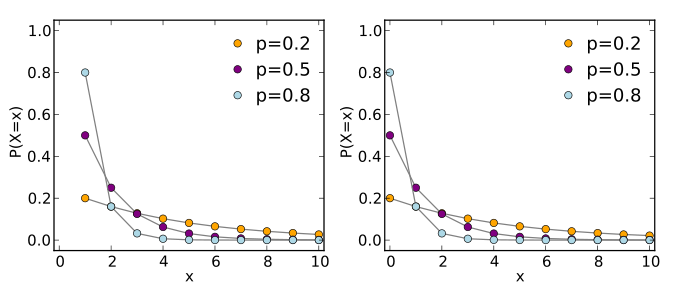
\includegraphics[scale = 0.25]{geometric_pmf}\\
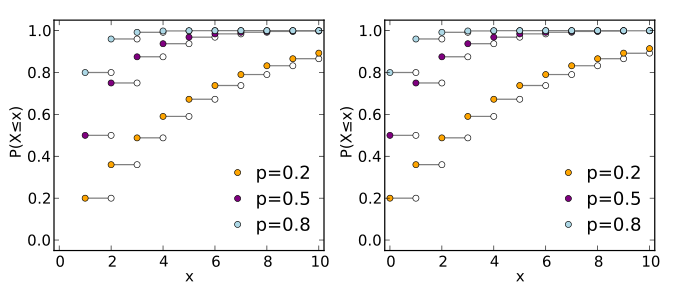
\includegraphics[scale = 0.25]{geometric_cdf}
\caption{\textbf{Top Panel}: The PMF of the geometric distribution under both parameterizations \textbf{Bottom Panel}: The CDF of the geometric distribution under both parameterizations}
\end{figure}
\end{center}
\end{frame}

\subsection{Transformations of Random Variables}
\begin{frame}{Transformations of Random Variables using the Change of Variables Formula}
Assume that $X$ has a pdf $f_{X}(x)$ and that $Y = g(X)$ where g is a monotone function. Suppose that  $f_{X}(x)$ is continuous on $\mathcal{X}$, and that $g^{-1}$ has a continuous derivative on $\mathcal{Y}$ where $\mathcal{X}, \mathcal{Y}$ are such that $\mathcal{X} = \{x: f_{X}(x) > 0\}$ and $\mathcal{Y} = \{y: y = g(x)\}$. Then the pdf of $Y$ is given as follows:
\begin{align*}
f_{Y}(y) = f_{X}(g^{-1}(y))|\frac{\mathrm{d}}{\mathrm{d}y}g^{-1}(y)|
\end{align*}
\end{frame}
 
\begin{frame}{Transformations of Random Variables - Example}
Assume that $X\sim f_{X}(x) = 1$ i.e. $X\sim\mathrm{Uniform}(0, 1)$. Furthermore, $Y = -\log(X)$. What is the PDF of $Y$?
\newline 

First note that $g(X)  = Y  = -\log (X) \rightarrow g^{-1}(Y) = e^{-Y}$. Therefore, using the formulation from earlier:
\begin{align*}
f_{Y}(y) = 1 \cdot |-e^{-Y}| = e^{-Y} \\
Y \sim \mathrm{Exponential}(\lambda = 1)
\end{align*}
\end{frame}

\begin{frame}{Transformations of Random Variables - Exercise}
Assume that $X\sim \mathrm{Normal}(0,1)$. Let $Y = X^{2}$. What is the distribution of $Y$?
\newline

The PDF of the standard normal distribution is given as follows:
\begin{align*}
f_{X}(x) = \frac{1}{\sqrt{2\pi}} \exp\{-\frac{x^{2}}{2}\}
\end{align*}
\end{frame}

\begin{frame}{Transformations of Random Variables - Exercise Cont.}
Consider that $Y = g(X) = X^{2} \rightarrow g^{-1}(Y) = \mp \sqrt{Y}$. Hence, consider that we can partition the support of $X$ into two pieces $S_{1} = (-\infty, 0)$ and $S_{2} = (0, \infty)$ where the function $g(X)$ is monotone. Note that $\mathcal{Y} = (0, \infty)$. Use the change of variables formulation over the two partitions and sum:
\begin{align*}
f_{Y}(y) &= \frac{1}{\sqrt{2\pi}}\exp\{\frac{-(-\sqrt{Y})^{2}}{2}\}|-\frac{1}{2\sqrt{y}}| + \frac{1}{\sqrt{2\pi}}\exp\{\frac{-(\sqrt{Y})^{2}}{2}\}|\frac{1}{2\sqrt{y}}| \\
&= \frac{1}{\sqrt{2\pi}}\frac{1}{\sqrt{Y}}\exp\{\frac{-y}{2}\}
\end{align*}
Hence, we get that $Y \sim \chi^{2}_{df = 1}$
\end{frame}

\begin{frame}{Expectations and Variances of Random Variables}
The expectation of any random variable can be computed as follows:
\begin{itemize}
\item{$\mathbb{E}[g(X)] = \int_{-\infty}^{\infty}g(x)f_{X}(x) \mathrm{d}x$ when $X$ is continuous}
\item{$\mathbb{E}[g(X)] = \sum_{x\in\mathcal{X}}g(x)f_{X}(x) = \sum_{x\in\mathcal{X}}g(x)\mathbb{P}(X = x)$ when $X$ is discrete}
\end{itemize}
The variance can be computed using the expectations as follows:
\begin{align*}
\mathbb{V}[X]  = \mathbb{E}[X^{2}] - (\mathbb{E}[X])^{2}
\end{align*}
You will need to do some calculus to find each of these quantities
\end{frame}

\begin{frame}{Kernel Tricks for Computing Expectations - Example}
If we say that $X\sim\mathrm{Exponential}(\lambda)$, with PDF $f_{X}(x) = \lambda\exp\{-\lambda x\}$. In order to find $\mathbb{E}[X]$, you must find:
\begin{align*}
\mathbb{E}[X] = \int_{0}^{\infty} x\lambda\exp\{-\lambda x\} \mathrm{d}x
\end{align*}
\begin{itemize}
\item{Integration by parts}
\item{Something a bit more clever?}
\end{itemize}
\end{frame}

\begin{frame}{Kernel Tricks for Computing Expectations - Example Cont.}
First, notice that if we say that $X\sim\mathrm{Gamma}(\alpha, \beta)$ and PDF $g_{X}(x) = \frac{\beta^{\alpha}}{\Gamma(\alpha)} x^{\alpha - 1} e^{-\beta x}$
\newline

In instances when $\alpha = 1$ then this an Exponential random variable with $\lambda = \beta$. 
\newline 

The integrand from the previous slide, is \emph{almost} like a Gamma PDF with $\alpha = 2$. Hence, you can complete it by some clever multiplication and division:
\begin{align*}
\mathbb{E}[X] = \frac{\Gamma(2)}{\lambda^{2}}\int_{0}^{\infty}\frac{\lambda^{2}}{\Gamma(2)} x^{2-1}\lambda\exp\{-\lambda x\} \mathrm{d}x = \frac{1}{\lambda} \cdot 1 = \frac{1}{\lambda}
\end{align*}
\end{frame}

\begin{frame}{Kernel Tricks for Computing Expectations - Exercise}
Use the kernel trick for Exponential random variables to find $\mathbb{V}[X]$
\end{frame}


\begin{frame}{Kernel Tricks for Computing Expectations - Exercise}
The first step in this process is to find $\mathbb{E}[X^{2}]$ which you can calculate using the kernel trick as follows:
\begin{align*}
\mathbb{E}[X^{2}] = \frac{\Gamma(3)}{\lambda^{3}}\int_{0}^{\infty}\frac{\lambda^{3}}{\Gamma(3)} x^{2-1}\lambda\exp\{-\lambda x\} \mathrm{d}x = \frac{2}{\lambda^{2}} \cdot 1 = \frac{2}{\lambda^{2}}
\end{align*}
Plug this result into the variance formula presented earlier using the expectation from earlier:
\begin{align*}
\mathbb{V}[X] = \frac{2}{\lambda^{2}} - \frac{1}{\lambda^{2}} = \frac{1}{\lambda^{2}}
\end{align*}

\textbf{Note}: You will not have to use a lot of integration here. Always try these tricks first
\end{frame}

\begin{frame}{Properties of Expectations and Variances}
Assume a random variable $X$ and $a$ is a scalar constant, then:
\begin{align*}
\mathbb{E}[aX] &= a \mathbb{E}[X] \\
\mathbb{V}[aX] &= a^{2} \mathbb{V}[X]
\end{align*}
Variances also have nice properties. Consider two random variables $X$ and $Y$.
\begin{align*}
\mathbb{V}[X \mp Y] = \mathbb{V}[X] + \mathbb{V}[Y] \mp 2\mathbb{C}(X,Y)
\end{align*}
These extend to multivariate random variables as well.
\end{frame}

\subsection{A Gentle Introduction to Distribution Theory}

\begin{frame}{Discrete Distributions}
A random variable $X$ is \emph{discrete} if the range of $X$, the sample space, is countable. In most situations, the random variable has integer valued outcomes
\newline

Some examples of discrete distributions:
\begin{itemize}
\item{Binomial Distribution}
\item{Poisson Distribution}
\item{Negative Binomial Distribution}
\end{itemize}
\end{frame}


\begin{frame}{Binomial Distribution}
This distribution counts the the number of successes in $n$ independent trials all with the same fixed probability $p$ of success
\begin{align*}
X &\sim \mathrm{Binomial}(n, p) \\
P(X  = x) &= \frac{n!}{x!(n-x)!} p^{x}(1-p)^{n-x} \\
\mathbb{E}[X] &= np \\
\mathbb{V}[X] &= n p (1-p)
\end{align*}
\end{frame}

\begin{frame}{Poisson Distribution}
This distribution is used for counting the number of events over some time horizon based on an intensity parameter $\lambda$
\begin{align*}
X &\sim \mathrm{Poisson}(\lambda)\\
P(X = x) &= \frac{\exp^{-\lambda}\lambda^{x}}{x!}\\
\mathbb{E}[X] &= \mathbb{V}[X] = \lambda
\end{align*}
\end{frame}

\begin{frame}{Poisson Distribution - Exercise}
Prove that $\mathbb{E}[X] = \lambda$ if $X\sim\mathrm{Poisson}(\lambda)$
\end{frame}

\begin{frame}{Poisson Distribution - Exercise Cont.}
We need to compute the following:
\begin{align*}
\mathbb{E}[X] &= \sum_{x = 0}^{\infty}x \frac{\exp^{-\lambda}\lambda^{x}}{x!} \\
&= \lambda \exp\{-\lambda\} \sum_{x = 1}^{\infty}\frac{\lambda^{x-1}}{(x-1)!} 
\end{align*}
Now recognize the following result from the Taylor series expansion on $\exp\{y\} = \sum_{i=0}^{\infty}\frac{y^{i}}{i!}$. Use this result with a clever substitution:
\begin{align*}
\lambda \exp\{-\lambda\} \exp\{\lambda\} = \lambda
\end{align*}
\end{frame}

\begin{frame}{Negative Binomial Distribution}
This distribution counts the the number successful trials $k$ that occur before the $r$th failed trial, where each trial has fixed probability $p$ of success
\begin{align*}
X &\sim \mathrm{NB}(p, r) \\
P(X  = n) &= \frac{(k+r - 1)!}{k!(r-1)!} p^{k}(1-p)^{r} \\
\mathbb{E}[X] &= \frac{pr}{1-p} \\
\mathbb{V}[X] &= \frac{p r}{(1-p)^2}
\end{align*}

Is highly related to the Poisson and Gamma Distributions
\end{frame}



\begin{frame}{Continuous Distributions}
A random variable $X$ is \emph{continuous} if the range of $X$, the sample space, takes on an uncountably infinite number of values. In most instances the random variable has real-valued outcomes. 
\newline

Some examples of Continuous Distributions
\begin{itemize}
\item{Normal Distribution}
\item{Chi-Squared Distribution}
\item{Exponential Distribution}
\item{Gamma Distribution}
\item{Inverse-Gamma Distribution}
\item{Student-t Distribution}
\item{F Distribution}
\item{Beta Distribution}
\end{itemize}
\end{frame}

\begin{frame}{Normal Distribution}
A random variable $X\sim\mathrm{Normal}(\mu, \sigma^{2})$ with PDF:
\begin{align*}
f_{X}(x) = \frac{1}{\sqrt{2\pi\sigma^{2}}}\exp\{-\frac{(x-\mu)^{2}}{2\sigma^{2}}\}
\end{align*}
We also sometimes express this in terms of a \emph{precision} parameter, rather than a variance, $X\sim\mathrm{Normal}(\mu, \phi^{-1})$ which becomes useful when performing Bayesian inference.  If $Z \sim \mathrm{Normal}(0, 1)$ then the distribution of $Z$ is standard normal.\\
\end{frame}

\begin{frame}
\frametitle{Chi-Squared Distribution}
If $Z_1$, $Z_2, \hdots, Z_k$ are independent, standard normal random variables, then 

$$\sum_{j = 1}^k Z_j^2 \sim \chi^2_k$$

follows a Chi-Squared distribution with $k$ degrees of freedom.  This is a special case of the Gamma distribution, discussed on the next slide.  


\end{frame}

\begin{frame}{Gamma Distribution}
A random variable $X\sim\mathrm{Gamma}(\alpha, \beta)$ with PDF:
\begin{align*}
f_{X}(x) &= \frac{\beta^{\alpha}}{\Gamma(\alpha)}x^{\alpha-1}\exp\{-x\beta\} \\
\mathbb{E}[X] &= \frac{\alpha}{\beta} \\
\mathbb{V}[X] &= \frac{\alpha}{\beta^{2}} \\
&\alpha, \beta > 0 \\
&x \in (0, \infty)
\end{align*} 
\end{frame}

\begin{frame}{Gamma Distribution  - Important Properties}
Here are some important tricks that will be useful in \textbf{711} and \textbf{601}
\begin{itemize}
\item{if $\alpha = 1$ and then $X\sim\mathrm{Exponential}(\lambda = \beta)$}
\item{if $\alpha = \frac{\nu}{2}$ and $\beta = \frac{1}{2}$ then $X\sim\chi^{2}_{\nu}$}
\item{if $X\sim\mathrm{Gamma}(\alpha_{1}, \beta)$ and $Y\sim\mathrm{Gamma}(\alpha_{2}, \beta)$ then $X+Y\sim\mathrm{Gamma}(\alpha_{1}+\alpha_{2}, \beta)$}
\item{if $X\sim\mathrm{Gamma}(k, \theta)$, then $\frac{1}{X}\sim\mathrm{Inverse-Gamma}(k, \frac{1}{\theta})$}
\end{itemize}
\end{frame}

\begin{frame}{Student's-$t$ Distribution}
A random variable $T$ follows a Student's-$t$ distribution if
\begin{align*}
T & = \frac{Z}{\sqrt{V/\nu}},\\
Z &\sim N(0, 1),\\
V &\sim \chi^2_{\nu}
\end{align*} 

and $Z$ and $V$ are independent.
\end{frame}

\begin{frame}{$F$ Distribution}
A random variable $X$ follows a $F$-distribution with numerator degrees of freedom $\nu_1$ and denominator degrees of freedom $\nu_2$ if
\begin{align*}
X &= \frac{V_1 / \nu_1}{V_2 / \nu_2}
\end{align*} 

where $V_1$ and $V_2$ are independent chi-squared random variables with degrees of freedom equal to $\nu_1$ and $\nu_2$ respectively.
\end{frame}

\begin{frame}{Beta Distribution}
A random variable $X\sim\mathrm{Beta}(\alpha, \beta)$ with PDF:
\begin{align*}
f_{X}(x) &= \frac{\Gamma(\alpha + \beta)}{\Gamma(\alpha)\Gamma(\beta)}x^{\alpha-1}(1-x)^{\beta - 1} \\
\mathbb{E}[X] &= \frac{\alpha}{\alpha + \beta} \\
\mathbb{V}[X] &= \frac{\alpha \beta}{(\alpha + \beta)^{2}(\alpha + \beta + 1)} \\
&\alpha, \beta > 0 \\
&x \in (0, 1)
\end{align*} 

Very useful for eliciting probability distributions for proportions.\\~\\

\href{https://en.wikipedia.org/wiki/Relationships_among_probability_distributions}{Cool distributional relationships}
\end{frame}

\begin{frame}{Exponential Families}
A family of PDFs and PMFs are called exponential family distributions if they can be expressed in the form:
\begin{align*}
f_{X}(x|\theta) &= h(x) c(\theta)\exp\{\sum_{i = 1}^{k}\omega_{i}(\theta)t_{i}(x)\}\\
\end{align*}
Where:
\begin{align*}
h(x) &\geq 0 \\
c(\theta) &\geq 0 \\
\omega_{1}(x),&\ldots,\omega_{k}(x) \in \mathbb{R}\\
t_{1}(x),&\ldots t_{k}(x) \in \mathbb{R}\\
\end{align*}
While this may not seem important yet, exponential family distributions have some really, really nice properties that make their applications extremely widespread (\textbf{732})

\end{frame}

\begin{frame}{Exponential Families - Example}
Consider the binomial PMF for a random variable $X\sim\mathrm{Binomial}(n, p)$
\begin{align*}
P(X = x) = \frac{n!}{(n - x)!x!} p^{x} (1-p)^{n-x}
\end{align*}
This is an exponential family PMF. We can show this by re-expressing terms:
\begin{align*}
P(X = x) &= \frac{n!}{(n - x)!x!} (1-p)^{n} \exp\{x\log(\frac{p}{1-p}) \} \\
h(x) &= \frac{n!}{(n - x)!x!} \mathbb{I}_{x = 0, \ldots, n}\\
c(p) &= (1-p)^{n} \\
\omega_{1}(p) &= \log(\frac{p}{1-p}) \\
t_{1}(x) &= x \\
\end{align*}
\end{frame}

\begin{frame}{Exponential Families - Exercise}
Consider the following normal PDF for $X\sim\mathrm{Normal}(\mu, \sigma^{2})$
\begin{align*}
f_{X}(x|\mu, \sigma^{2}) = \frac{1}{\sqrt{2\pi\sigma^{2}}}\exp\{-\frac{(x-\mu)^{2}}{2\sigma^{2}}\} 
\end{align*}
Show that this is an exponential family PDF
\end{frame}

\begin{frame}{Exponential Families - Exercise Cont.}
Consider the following PDF
\begin{align*}
f_{X}(x|\mu, \sigma^{2}) = \frac{1}{\sqrt{2\pi\sigma^{2}}}\exp\{-\frac{(x-\mu)^{2}}{2\sigma^{2}}\} 
\end{align*}
Expanding the exponential yields the following
\begin{align*}
f_{X}(x|\mu, \sigma^{2}) &= \frac{1}{\sqrt{2\pi\sigma^{2}}}\exp\{-\frac{\mu^{2}}{2\sigma^{2}}\} \exp\{ -\frac{x^{2}}{2\sigma^{2}} + \frac{\mu x}{\sigma^{2}}\}\\
h(x) &= 1\\
c(\mu, \sigma)  &= \frac{1}{\sqrt{2\pi\sigma^{2}}}\exp\{\frac{-\mu^{2}}{\sigma^{2}}\}; \mu\in\mathbb{R}\>\>\>\sigma^{2}>0\\
\omega_{1}(\mu, \sigma) &= \frac{1}{\sigma^{2}}\>\>\>\omega_{2} = \frac{\mu}{\sigma^{2}} \\
t_{1}(x) &= \frac{-x^{2}}{2} \>\>\> t_{2}(x) = x
\end{align*}
\end{frame}

\section{Multivariate Random Variables}
\begin{frame}{Random Vectors}
The basic definition of a \emph{Random Vector} carries over from the definition of a random variable presented earlier. In the later half, you'll see this is a more general setting. Here we will emphasize bi-variate examples.
\begin{center}
An $n$ dimensional random vector is a function from a sample space into $\mathbb{R}^{n}$, $n$-dimensional euclidean space
\end{center}
An example of a 2-dimensional random vector is as follows:
\begin{center}
Recall that two dice being rolled have a sample space of 36 points. Associate the random variables $X$ and $Y$ with the sample space as follows:
\end{center}
\begin{align*}
X = D_{1} + D_{2} \\
Y = |D_{1}-D_{2}|
\end{align*}
In this way, the pair $(X, Y)$ define a bi-variate random vector
\end{frame}

\begin{frame}{Distribution Functions for Multivariate Random Variables}

There are three types of distribution functions that we will cover:
\begin{itemize}
\item{Joint Distribution}
\item{Marginal Distribution}
\item{Conditional Distribution}
\end{itemize}
\end{frame}

\begin{frame}{Joint Distribution - Bivariate Case}
\textbf{Joint PDF}:
A function $f(x, y)$ from $\mathbb{R}^{2} \rightarrow \mathbb{R}$ is called a joint PDF of the random vector $(X, Y)$ if for every $A \subset \mathbb{R}^{2}$
\begin{align*}
\mathbb{P}((X, Y) \in A) = \int_{A}\int f_{X, Y}(x, y) \mathrm{d}x\mathrm{d}y
\end{align*} 

\textbf{Joint PMF}:
The function $f(x, y)$ from $\mathbb{R}^{2} \rightarrow \mathbb{R}$ defined by $f_{X, Y}(x, y) = \mathbb{P}(X = x, Y = y)$ is the joint PMF of $X, Y$. Then for every $A \subset \mathbb{R}^{2}$
\begin{align*}
\mathbb{P}((X, Y)\in A) = \sum_{(x, y)\in A}f_{X, Y}(x, y)
\end{align*}
\end{frame}

\begin{frame}{Joint Distribution - Exercise}
Assume that $X$ and $Y$ have the joint PDF:
\begin{align*}
    f_{X,Y}(x, y) &= 4xy \\
    0<&x<1\\
    0<&y<1
\end{align*}
Find $P(Y < X)$
\end{frame}
 
\begin{frame}{Joint Distribution - Exercise Cont.}
We can set up the double integral required for this probability as follows:
\begin{align*}
p(Y<X) &= \int_{0}^{1}\int_{0}^{x}4 xy \mathrm{d}y\mathrm{d}{x} \\
&= \int_{0}^{1}[4x \frac{y^{2}}{2}]\bigg|_{0}^{x}\mathrm{d}{x}\\
&= \int_{0}^{1}2x^{3}\mathrm{d}{x} = \frac{1}{2}
\end{align*}
\end{frame}
 
\begin{frame}{Marginal Distribution}
Given the joint PDF or joint PMF, you can find the marginal PDF or PMF:

\textbf{Marginal PDF}:
\begin{align*}
f_{X}(x) = \int_{Y} f_{X, Y}(x, y) \mathrm{d}y
\end{align*}
\textbf{Marginal PMF}:
\begin{align*}
f_{Y}(y) = \sum_{x} f_{X, Y}(x, y) 
\end{align*}
\end{frame}

\begin{frame}{Conditional Distribution}
Assume that $X, Y \sim f_{X,Y}(x, y)$, then we can employ Bayes' rule for distributions:
\begin{align*}
f_{X|Y}(x|y) = \frac{f_{X, Y}(x, y)}{f_{Y}(y)}
\end{align*}
\end{frame}

\begin{frame}{Multivariate Distributions - Exercise}
Assume that $(X, Y)$ are a continuous random vector with joint pdf given by:
\begin{align*}
f_{X, Y}(x, y) = \exp\{-y\}\>\>\> 0<x<y<\infty
\end{align*}
Find the marginal distribution of $X$ and the conditional distribution $Y|X$
\end{frame}



\begin{frame}{Multivariate Distributions - Example Cont.}
We start by finding the marginal distribution of $X$:
\begin{align*}
f_{X}(x) &= \int_{x}^{\infty} \exp\{ -y \}\mathrm{d}y = e^{-x} \\
X&\sim\mathrm{Exponential}(\lambda = 1)
\end{align*}
Now use the results on conditional distributions given earlier, to find:
\begin{align*}
f_{Y|X}(y|x) =  \frac{f_{X, Y}(x, y)}{f_{X}(x)} = \frac{\exp\{ -y\}}{\exp{\{ -x\}}} \mathbb{I}(x<y)
\end{align*}
\end{frame}

\begin{frame}{Total Expectation and Total Variance Laws}
In many examples, you are interested in marginal moments from conditional distributions. Your first option of course if to find the joint distribution, do some marginalization and then integrate, but I do not like calculus so \textbf{instead}:
\begin{align*}
\mathbb{E}[Y] &= \mathbb{E}[\mathbb{E}[Y|X]] \\
\mathbb{V}[Y] &= \mathbb{V}[\mathbb{E}[Y|X]] + \mathbb{E}[\mathbb{V}[Y|X]]
\end{align*}
\end{frame}

\begin{frame}{Total Expectation and Total Variance Laws - Example}
Assume that we have the following relationship:
\begin{align*}
X|N &\sim \mathrm{Binomial}(N, p) \\
N &\sim\mathrm{Negative Binomial}(\tau = \frac{1}{1+\beta}, r = 1)
\end{align*}
\newline

Find $\mathbb{E}[X]$ and $\mathbb{V}[X]$
\newline

\textbf{Tip}: that $\mathbb{E}[N] = \frac{r\tau}{1-\tau}$ and $\mathbb{V}[N] = \frac{\tau r}{(1-\tau)^{2}} $
\end{frame}

\begin{frame}{Total Expectation and Total Variance Laws - Example Cont.}
First, we iterate to find the expectation
\begin{align*}
\mathbb{E}[X] &= \mathbb{E}[\mathbb{E}[X|N]]\\
&= \mathbb{E}[Np]\\
&= p\frac{\frac{1}{1+\beta}}{1-\frac{1}{1+\beta}}\\
&= \frac{p}{\beta}
\end{align*}
Next, we proceed with finding the variance
\begin{align*}
\mathbb{V}[X] &= \mathbb{E}[\mathbb{V}[X|N]] + \mathbb{V}[\mathbb{E}[X|N]] \\
&= \mathbb{E}[Np(1-p)] + \mathbb{V}[Np]\\
&= \frac{p(1-p)}{\beta} + p^{2}\frac{1+\beta}{\beta^{2}}
\end{align*}
\end{frame}

\begin{frame}{Total Expectation and Total Variance Laws - Exercise}
\begin{align*}
X|P&\sim\mathrm{Binomial}(n, P) \\
P &\sim\mathrm{Beta}(a, b)
\end{align*}
\newline
Find the $\mathbb{E}[X]$ and $\mathbb{V}[X]$

\textbf{Tip}:
\begin{align*}
\mathbb{E}[P] &= \frac{a}{a+b} \\
\mathbb{V}[P] &= \frac{ab}{(a+b)^{2}(a+b+1)}
\end{align*}
\end{frame}


\begin{frame}{Total Expectation and Total Variance Laws - Exercise Cont.}
We can start by finding the marginal expectation first:
\begin{align*}
\mathbb{E}[X] &= \mathbb{E}[\mathbb{E}[X|P]] = \mathbb{E}[nP] = n \mathbb{E}[P] = n \frac{a}{a+b}
\end{align*}
And then the marginal variance:
\begin{align*}
\mathbb{V}[X] &= \mathbb{V}[\mathbb{E}[X|P]] + \mathbb{E}[\mathbb{V}[X|P]]\\
&= \mathbb{V}[nP] + \mathbb{E}[nP(1-P)]\\
&= n^{2}\mathbb{V}[P] + n\mathbb{E}[P - P^{2}] \\
& = n^{2} \frac{ab}{(a+b)^{2}(a+b+1)} + n \frac{a}{a+b} \\ &- n (\frac{ab}{(a+b)^{2}(a+b+1)}) - n (\frac{a}{a+b})^{2}\\
& = n \frac{ab(a+b+n)}{(a+b)^{2}(a+b+1)}
\end{align*}
\end{frame}

\section{Random Matrices and Multivariate Statistics}
\begin{frame}
\frametitle{Random Vectors}
If we have $d$ random variables $X_1, X_2, \hdots, X_d$, each defined on the real line, we can write them as the $d$ dimensional column vector $$\mathbf{X} = (X_1, \cdots X_d)^T$$

which we call a $d$-dimensional \textbf{random vector}.  The joint distribution function of the random vector $\mathbf{X}$ is

\begin{align*}
F_X(\mathbf{x}) &= F_X(x_1, \hdots, x_d) \\
&= P(X_1 \leq x_1, \hdots, X_d \leq x_d)\\
&= P(\mathbf{X} \leq \mathbf{x})
\end{align*}

If $F_X$ is absolutely continuous, then the joint density function $f_X$ of $\mathbf{X}$ is

$$f_X(\mathbf{x}) = f_X(x_1, \hdots, x_d) = \frac{\partial ^d F_X(x_1, \hdots, x_d)}{\partial x_1 \cdots \partial x_d}$$
\end{frame}

\begin{frame}
\frametitle{Random Vectors}
To find the marginal density of a subset of the $d$ variables, you can just integrate the others out.  For example, if we have a joint bivariate density $f_{X_1,X_2}(x_1, x_2)$, then 

$$f_{X_1}(x_1) = \int_{-\infty}^{\infty} f_{X_1,X_2}(x_1, x_2) dx_2 \qquad f_{X_2}(x_2) = \int_{-\infty}^{\infty} f_{X_1,X_2}(x_1, x_2) dx_1$$

The components of a random vector $\mathbf{X}$ are \textbf{independent} if the joint distribution function is a product of the marginal distribution functions

$$F_X(\mathbf{x}) = \prod_{i=1}^d F_i(x_i)$$

In addition, the joint density is the product of marginals

$$f_X(\mathbf{x}) = \prod_{i=1}^d f_i(x_i)$$
\end{frame}

\begin{frame}
\frametitle{Expectation and Covariance}
If $\mathbf{X}$ is a random vector with values in $\mathbb{R}^d$, then its expected value is given by the $d$ dimensional vector

$$\mathbf{\mu}_X = E(\mathbf{X}) = (E(X_1), \cdots, E(X_d)) = (\mu_1, \cdots, \mu_d)^T$$

and the $d \times d$ \textbf{covariance matrix} of $\mathbf{X}$ is 

\begin{align*}
\mathbf{\Sigma}_{XX} &= \text{cov}(\mathbf{X}, \mathbf{X}) \\
&= E[(\mathbf{X} - \mathbf{\mu}_X)(\mathbf{X} - \mathbf{\mu}_X)^T]\\
&= E[(X_1 - \mu_1, \cdots, X_d - \mu_d) (X_1 - \mu_1, \cdots, X_d - \mu_d)^T]\\
&= 
\begin{pmatrix}
    \sigma_1^2 & \sigma_{12} & \dots  & \sigma_{1d}\\
    \sigma_{21} & \sigma_2^2  & \dots  & \sigma_{2d}\\
    \vdots & \vdots  & \ddots & \vdots \\
    \sigma_{d1} & \sigma_{d2}  & \dots  & \sigma_d^2
\end{pmatrix}
\end{align*} 
\end{frame}

\begin{frame}
\frametitle{Correlation Matrix}
The \textbf{correlation matrix} of $\mathbf{X}$ can be obtained by from $\mathbf{\Sigma}_{XX}$ by dividing the $i$th row by $\sigma_i$ and the $j$th column by $\sigma_j$.  The $d \times d$ matrix is then

$$P_{XX} = \begin{pmatrix}
    1 & \rho_{12} & \dots  & \rho_{1d}\\
    \rho_{21} & 1  & \dots  & \rho_{2d}\\
    \vdots & \vdots  & \ddots & \vdots \\
    \rho_{d1} & \rho_{d2}  & \dots  & 1
\end{pmatrix}$$

where 

$$\rho_{ij} = \rho_{ji} = \begin{cases}
\frac{\sigma_{ij}}{\sigma_i \sigma_j} & i \neq j\\
1 & \text{otherwise}
\end{cases}
$$

is the pairwise correlation coefficient between $X_i$ and $X_j$.  The correlation coefficient will always lie between $-1$ and $1$ and is a measure of association between $X_i$ and $X_j$.
\end{frame}

\begin{frame}
\frametitle{Linear Functions of Random Vectors}
If $\mathbf{Y}$ is a linear function of $\mathbf{X}$ such that

$$\mathbf{Y} = \mathbf{AX} + \mathbf{b}$$

the mean vector and covariance matrix of $\mathbf{Y}$ is given by

\begin{align*}
\mathbf{\mu}_Y &= \mathbf{A\mu}_x + \mathbf{b}\\
\mathbf{\Sigma}_{YY} &= \mathbf{A\Sigma_{XX}A}^T
\end{align*}
\end{frame}

\begin{frame}
\frametitle{Multivariate Normal Distribution}
The form of the multivariate normal looks similar to that of the univariate normal.  A random $d$ vector $\mathbf{X}$ follows a multivariate normal distribution with mean vector $\mu$ and positive definite symmetric covariance matrix $\mathbf{\Sigma}$ if it has the density function

$$f(\mathbf{x}|\mu, \mathbf{\Sigma}) = (2\pi)^{-d/2}|\mathbf{\Sigma}|^{-1/2} e^{-\frac{1}{2} (\mathbf{x} - \mathbf{\mu})^T \mathbf{\Sigma}^{-1}(\mathbf{x} - \mathbf{\mu})}$$

We notationally denote a $d$ dimensional normal distribution as 

$$\mathbf{X} \sim N_d(\mu, \mathbf{\Sigma})$$
\end{frame}

\begin{frame}
\frametitle{Multivariate Normal Distribution}
The \textbf{Mahalanobis distance} from $\mathbf{x}$ to $\mathbf{\mu}$ is given by the quadratic form

$$\Delta = \sqrt{(\mathbf{x} - \mathbf{\mu})^T \mathbf{\Sigma}^{-1}(\mathbf{x} - \mathbf{\mu})}$$

An important result is that a random vector $\mathbf{X}$ follows a multivariate distribution if and only if every linear function of $\mathbf{X}$ follows a univariate normal distribution.
\vspace{5mm}

In linear models, we often assume that $\mathbf{\Sigma} = \sigma^2\mathbf{I_d}$, in which case the density function reduces to

$$f(\mathbf{x}|\mu, \sigma) = (2\pi \sigma)^{-d/2} e^{-\frac{1}{2} (\mathbf{x} - \mathbf{\mu})^T (\mathbf{x} - \mathbf{\mu})}$$
\end{frame}

\begin{frame}
\frametitle{Partitioned Random Vectors}
Suppose we have two random vectors $\mathbf{X}$ and $\mathbf{Y}$, where $\mathbf{X}$ has $d_1$ components and $\mathbf{Y}$ had $d_2$ components.  Let $\mathbf{Z}$ be the random $d_1 + d_2$ vector

$$\mathbf{Z} = \begin{pmatrix} \mathbf{X} \\ \mathbf{Y} \end{pmatrix}$$

Then the expected value and covariance matrix of $\mathbf{Z}$ is given by 
\begin{align*}
\mathbf{\mu}_Z &= E[\mathbf{Z}] = \begin{pmatrix} E[\mathbf{X}] \\ E[\mathbf{Y}] \end{pmatrix} = \begin{pmatrix} \mathbf{\mu}_X \\ \mathbf{\mu}_Y \end{pmatrix}\\
\mathbf{\Sigma}_{ZZ} &= \begin{pmatrix} cov(\mathbf{X}, \mathbf{X}) & cov(\mathbf{X}, \mathbf{Y}) \\ cov(\mathbf{Y}, \mathbf{X}) & cov(\mathbf{Y}, \mathbf{Y})  \end{pmatrix}\\
&= \begin{pmatrix}
\mathbf{\Sigma_{XX}} & \mathbf{\Sigma}_{XY}\\
\mathbf{\Sigma}_{YX} & \mathbf{\Sigma}_{YY}
\end{pmatrix}
\end{align*}

where $\mathbf{\Sigma}_{XY} = \mathbf{\Sigma}_{YX}^T$. 
\end{frame}

\begin{frame}
\frametitle{Marginal/Conditional Normal Distribution}
The marginal distribution of $\mathbf{Y}$ is

$$\mathbf{Y} \sim N_{d_2}(\mu_y, \mathbf{\Sigma}_{YY}$$

The conditional distribution of $\mathbf{Y}$ given that $\mathbf{X} = \mathbf{x}$ is multivariate normal with mean vector and covariance matrix given by

\begin{align*}
\mu_{Y|X} &= \mu_Y + \mathbf{\Sigma}_{YX} \mathbf{\Sigma}_{XX}^{-1} (\mathbf{x} - \mu_X)\\
\mathbf{\Sigma}_{Y|X} &= \mathbf{\Sigma}_{YY} - \mathbf{\Sigma}_{YX}\mathbf{\Sigma}_{XX}^{-1}\mathbf{\Sigma}_{XY}
\end{align*}

\end{frame}

\begin{frame}
\frametitle{Wishart Distribution}
Given $n$ independent and identically distributed $d$ vectors

$$\mathbf{X}_i \sim N_d(\mu , \mathbf{\Sigma})$$

we say that the random positive-definite, symmetric matrix

$$ \mathbf{W} = \sum_{i = 1}^n \mathbf{X_i} \mathbf{X_i}^T$$

follows a \textbf{Wishart distribution} with $n$ degrees of freedom and matrix $\mathbf{\Sigma}$.  We denote the Wishart distribution by

$$\mathbf{W} \sim \mathcal{W}_d(n, \mathbf{\Sigma})$$

You can think of the Wishart as a randomly drawn covariance matrix multiplied by the degrees of freedom $n$, since $E[\mathbf{W}] = n\mathbf{\Sigma}$.  As $n \rightarrow \infty$, $\mathbf{W}/n \rightarrow \mathbf{\Sigma}$. 
\end{frame}

\begin{frame}
\frametitle{Properties of the Wishart Distribution}
\begin{enumerate}
\item Let $\mathbf{W}_j \sim \mathcal{W}_d(n_j, \mathbf{\Sigma})$ be independent.  Then $\sum_{j = 1}^m \mathbf{W}_j \sim \mathcal{W}_d(\sum_{j=1}^m n_j, \mathbf{\Sigma})$
\item Suppose $\mathbf{W} \sim \mathcal{W}_d(n, \mathbf{\Sigma})$ and let $\mathbf{A}$ be a constant matrix having full row rank.  Then $\mathbf{AWA}^T \sim \mathcal{W}_d(n, \mathbf{A\Sigma A}^T$).
\item  Suppose $\mathbf{W} \sim \mathcal{W}_d(n, \mathbf{\Sigma})$ and let $\mathbf{a}$ be a fixed $d$ dimensional vector.  Then $\mathbf{a}^T\mathbf{Wa} \sim (\mathbf{a}^T\mathbf{\Sigma a})\chi^2_n$.
\end{enumerate}

You can think of the Wishart as a multidimensional chi-square distribution.  If $\mathbf{W}$ follows a Wishart distribution, then $\mathbf{W}^{-1}$ follows an \textbf{inverse Wishart distribution}.
\end{frame}

\begin{frame}
\frametitle{Review Exercises}
Given that 
$$\mathbf{X} =  
\begin{pmatrix}
X_1\\
X_2\\
X_3
\end{pmatrix}
\sim N_3(\mathbf{\mu}, \mathbf{\Sigma}) 
$$

where

$$\mathbf{\mu} = 
\begin{pmatrix}
\phantom{-}0\\
\phantom{-}1\\
-1
\end{pmatrix}
\qquad 
\mathbf{\Sigma} =  
\begin{pmatrix}
3 & 0 & 1\\
0 & 1 & 0\\
1 & 0 & 2
\end{pmatrix}
$$

\begin{enumerate}

\item Find the correlation matrix $\rho$ of $\mathbf{X}$\\
\item Find the marginal distribution of $X_2$.\\

\item Find the marginal distribution of $\{X_1, X_3\}$.\\

\item Find the conditional distribution of $X_1|X_3 = -1$.\\

\item Find the conditional distribution of $X_1|\{X_2 = 1, X_3 = -1\}$\\

\item Are $\{X_1, X_3\}$ and $X_2$ independent?\\

\item Are $X_1 + X_2$ and $X_1 - X_2$ independent?\\  
\end{enumerate}

\end{frame}

\begin{frame}
\frametitle{Solutions}
\begin{enumerate}
\item Find the correlation matrix $\rho$ of $\mathbf{X}$
$$\rho = \begin{pmatrix}
1 & 0 & 1/6\\
0 & 1 & 0\\
1/6 & 0 & 1
\end{pmatrix}$$

\item Find the marginal distribution of $X_2$.

$$ X_2 \sim N(1, 1)$$
\item Find the marginal distribution of $\{X_1, X_3\}$.

$$\{X_1, X_3\} \sim N\left(\begin{pmatrix} 0 \\ -1 \end{pmatrix} , \begin{pmatrix} 3 & 1 \\ 1 & 2 \end{pmatrix}\right)$$
\end{enumerate}
\end{frame}

\begin{frame}
\frametitle{Solutions}
\begin{enumerate}
\setcounter{enumi}{3}
\item Find the conditional distribution of $X_1|X_3 = -1$.
\vspace{5mm}

Using the conditional distribution formula, the conditional distribution of $\{X_1, X_2\}$ given $X_3 = -1$ is

\begin{align*}
\mu &= \begin{pmatrix} 0 \\ 1 \end{pmatrix} + \begin{pmatrix} 1 \\ 0 \end{pmatrix} (1/2) (0) =  \begin{pmatrix} 0 \\ 1 \end{pmatrix}\\
\mathbf{\Sigma} &= \begin{pmatrix} 3 & 0 \\0 & 1 \end{pmatrix} - \begin{pmatrix} 1 \\ 0 \end{pmatrix}(1/2) \begin{pmatrix} 1 \\ 0 \end{pmatrix}^T = \begin{pmatrix}5/2 & 0\\0 & 1\end{pmatrix}
\end{align*}

So looking at the marginal, the conditional distribution of $X_1$ is $N(0, 5/2)$.

\item Find the conditional distribution of $X_1|\{X_2 = 1, X_3 = -1\}$
$\{X_1, X_2\}$ given $X_3 = -1$ is

You can do this using the conditional distribution formula or note that $X_1$ is independent of $X_2$ (from the next question).  So the answer will be the same as above.
\end{enumerate}
\end{frame}

\begin{frame}
\frametitle{Solutions}
\begin{enumerate}
\setcounter{enumi}{5}

\item Are $\{X_1, X_3\}$ and $X_2$ independent?\\
Yes.  Since they are multivariate normally distributed and the pairwise correlation between $X_2$ and $\{X_1, X_3\}$ is 0, they are independent.

\item Are $X_1 + X_2$ and $X_1 - X_2$ independent?\\
No, the covariance between  $X_1 + X_2$ and $X_1 - X_2$ is nonzero (see next question).  Also, both terms involve $X_1$ and $X_2$ so there's no reason to expect them to be independent.  
\end{enumerate}
\end{frame}

\begin{frame}{Reference Guide}
\begin{itemize}
\item{\emph{Statistical Inference} - Casella and Berger}
\item{\emph{Mathematical Statistics} - Bickel and Doksum}
\item{\emph{A First Course in Bayesian Statistical Methods - Hoff}}
\item{\emph{Bayesian Computation with}\texttt{R} - Albert}
\end{itemize}
\end{frame}

\end{document}

